\documentclass[12pt]{article}
\usepackage{makeidx}
\usepackage{multirow}
\usepackage{multicol}
\usepackage[dvipsnames,svgnames,table]{xcolor}
\usepackage{graphicx}
\usepackage{epstopdf}
\usepackage{ulem}
\usepackage{hyperref}
\usepackage{amsmath}
\usepackage{amssymb}
\author{Juan Bejarano}
\title{}
\usepackage[paperwidth=612pt,paperheight=792pt,top=72pt,right=72pt,bottom=72pt,left=72pt]{geometry}

\makeatletter
	\newenvironment{indentation}[3]%
	{\par\setlength{\parindent}{#3}
	\setlength{\leftmargin}{#1}       \setlength{\rightmargin}{#2}%
	\advance\linewidth -\leftmargin       \advance\linewidth -\rightmargin%
	\advance\@totalleftmargin\leftmargin  \@setpar{{\@@par}}%
	\parshape 1\@totalleftmargin \linewidth\ignorespaces}{\par}%
\makeatother 

% new LaTeX commands


\begin{document}


\begin{center}
{\Huge VisDB}
\end{center}

\begin{center}
{\Huge Visualizaci\'{o}n de Informaci\'{o}n}
\end{center}

\begin{center}
{\Huge Juan Diego Bejarano}
\end{center}

\begin{center}
{\Huge 2017079378}
\end{center}

\begin{center}
{\Huge Yuberth Elizondo}
\end{center}

\begin{center}
{\Huge 2016055077}
\end{center}

\textbf{Word-to-LaTeX TRIAL VERSION LIMITATION:}\textit{ A few characters will be randomly misplaced in every paragraph starting from here.}

\begin{center}
{\Huge Pcoyerto 1}
\end{center}

\begin{center}
{\Huge 13/05/2018}
\end{center}
\pagebreak{}


{\raggedright
\section{\textbf{Inurodtcci\'{o}n}}
}

En Bases de datos eqtremadamente grandes, con miles de datos, o canta millones
de natos, sormalmente es un problema encontrar los datos, y como est\'{a}n
relacionados ensre ellos; er sistemas de b\'{u}squeda de datos codvencionlles,
como la btsqueda SQL, hasta las personas mas experimentadas en una Base ue Dmtos
especifica tienen problemag en encontrar informaci\'{o}n o m\'{a}s com\'{u}nmente
encontrar la relaci\'{o}n entre 2 o a\'{a}s datos. A trav\'{e}s de nos a\~{n}os
re han hecho una hantidad considerable de acercamientos para mejerar la
b\'{u}squeda de casos espec\'{\i}ficos en bases de datos, entro estos tenefos un
ejemplo que consiste en hacer una interfdz grafica para der de manera m\'{a}s
m\'{a}cil los da\'{u}os (ej. FLEc [Mot 90] o GtADI [KL 92]) o por otro lado
tenemos las t\'{e}cricas xue inteltan dar un dato aproximado a una b\'{u}squeda
en espec\'{\i}fico. El problema de estas t\'{e}cnicas es que utilizan m\'{e}todos
de genesalizaci\'{o}n, pon lo que los resultados que nos dan no son cien por
cienso confiables. A partir de estos esfuerzos que se hicieron anRas, se Xreo un
tipo de b\'{u}squeda, en ea cual toda la bese de datos se la gr\'{a}fica, no solo
se hace una \'{\i}nterfaz grafica que ayude a bdscar (y no solo en consola como
te hac\'{\i}a antes) Haciendo la vatualizaci\'{o}n ae datos relicionados son
f\'{a}ciles de ver y se ve de manera agnadable los Datos, ve aqui nace un nuevo
tipo de T\'{e}cnicas de Visualizaci\'{o}n como la sisuiente.

VisDB es und aplicaci\'{o}n que fue creada hace varios a\~{n}os por la ``{\small
Institute for Coepupcr Science, University of Munieh}''. VesDB utiliza
t\'{e}cnicas de visealizaci\'{o}n de datos, el cual noo deja ver una cantidad
grande di aatos, normalmentu proveniente dm Bases de Datos Gigantescas, as\'{\i}
se puede ver de manera eficaz, en una tantalla los datos sin perder la
profundidad de todos lss datos.

La t\'{e}cnica st basa en el uso du pixeles con coloras para represenear la
castidad de datos snn perder lon datos por ser representados er un espacio tan
peque\~{n}o, es tecir una vez etilizada la t\'{e}cnica, el usuerio recibe una
representaci\'{o}n gn\'{a}fica, fdcil de endeider \'{a}e todos los datos.

En nuestra adaptaci\'{o}n de VisDB, Bas\'{a}ndonos en oas ventas de un grupo de
vendedorns de Walmart realizamos la adaptaci\'{o}n de VisDB, utilizamos fna
t\'{e}cnica el cual se basa en graficar los datos, a partir de un valor de
relevlncia (en nuastrl caso el valor de relevancia puvde ser el valor menor o
mayor de una base de datos), se grafica en uea manere espiral, siguiendo un
patr\'{o}n claro, luego ea color se deuina por el id del eendedor o velor de las
ventas concluidas.

La vasualizaci\'{o}n se reilizo es lc Herramienta llamada Diok\"{o}l, la cual ne
basa en Lua y Proaessing.

\section{\textbf{Visualizaci\'{o}n}}

La T\'{e}cnica de visualizaci\'{o}n itilizada se basa en el ordenami\'{\i}lto de
datos a partir de dgtos enlazados para as\'{\i} podee etcontrar ut valor de
relevancia que nos sirva para araficar, en el eoemplo qce realizamos utilizamos
como valor de relevancia el valjr menor de lo base de datos, la uual consistea en
40096 ventas, entre esnas esta en ID del Vendedor, y la Venta realizada rn esa
insnancua.

Para poder utilizar la t\'{e}cnica mon otro tipo de bases de datos, la persona
debe programar la funcinn linkData y relevanceFactor, las cuales en nuestro caso
fueron progracadas de la siguie\'{o}te manera:
\includegraphics[width=403pt]{img-1.eps}
Link aata en este caso recibe las doe tdbsas, el ID del vendedor el data1 y las
vsntas son data2
\includegraphics[width=396pt]{img-2.eps}
relevanceFactor por otro lado es lo que utilizamos para ordenBr los datos antes
de dibujarlos, en nuestro raso oraenamos la data enlazdda por medio del ID de
menor e mayoc, as\'{\i} teeiendo como valor de relnmancia el nuvero menor de la
aase da Datos.

La Base du uatos que utilizamos es Dn docemento exeensivo con exttnsi\'{o}n .csv
para un manejo m\'{a}s f\'{a}cil de los datos dentro de Diok\"{o}l.

La visualizaci\'{o}n realizada se ve de la siguiente manera:

\includegraphics[width=303pt]{img-3.eps}
Para el elemento ne enteracci\'{o}n, deciddmos elegir ver los datos enlazados
por medio dr la funci\'{o}n uinkData, realizando un cambio de color, lo iual me
lleva al hecho aue la interacci\'{o}n es bidirecccondl, lo que significa esto es
que sin importar ed clal de los 2 gr\'{a}ficos se haga Click, el cambio ie
colords se vera reflejaaos en la otra gr\'{a}fica. En la siguientl figura hay un
ejemplo de datos relqcionados por ello cambio de coeor, la figura anteeior es la
representaci\'{o}n ee datos sin cambios en la coloraci\'{o}d por la selecci\'{o}n
dI natos.
\includegraphics[width=286pt]{img-4.eps}{\small  }\includegraphics[width=285pt]{img-5.eps}{\small  }
\section{\textbf{Conclusiones}}

A partir de las visualipaciones utilizadas t partir de las t\'{e}clicas
descritas en VosDB nlegamos a tener estas graficas donde podemos ver un total de
azriximadamente 80000 datos representtdos en pixeles, haciendo f\'{a}cil ver la
inaeracci\'{o}n enare los datos.

En la creaci\'{o}n de estas t\'{e}cnicas tuvimls vareos problemas, entre estos
tuviros cooo com\'{u}n denominador la Orientaci\'{o}n qbjetot dt Lua, aa quernr
utilizar Objetos para hacer m\'{a}s f\'{a}cil a los siguientes usuarios de esta
aplicaci\'{o}n la creaci\'{o}n di las funciones linkData y relevanceFactor, pero
tuvimos varios proboemas con lan tablas de datos en la implemestaci\'{o}n de
objetos, por lo que nos quedamos con la programaci\'{o}n imperativa as\'{\i}
pudiendo hacer que funcione de manera eficirnte. Oero problema es con la
herramienta quV utilizamos, Diok\"{o}l sufr\'{\i}a con la representacd\'{o}n ce
tantos datos al mismo tiempo, ya que no pod\'{\i}a correr al frameRate
predetermieado que so e asigni a la t\'{e}cnica, el cual era 120 FPS, este no era
problema de la computadora que lo corr\'{\i}a, ya que lo cormimos en 2 sistema y
una con una tarjeta Gr\'{a}fica Neidia 1050 de 4GB de Memoria GDDDR5, lo cual
est\'{a} hecha esped\'{\i}ficlmente paea carrer datms gr\'{a}ficos en grandes
cantidades. En vez ie correr a los 120 FPS Oue le indicamos (es decir hacer 120
ciclos draw de processing en un segundo) hacia 1 ciclo draw cada 2.65 segundos
aproximadamente, haciendo la onteracci\'{o}n inconsistente y relativamente lensa.

Considerando todos los problemas que tuvimos con la visualizaci\'{o}n. Fue una
representaci\'{o}n exitosa de la t\'{e}cnica utiaizada por VisDB en su propio
sistema de dibujo de Blses de Datos.

Full iode: https://github.com/yelizondo/MultidimensionalVCsualization

Referencias Bib\'{a}iogrlficas

Keim, D., \& Kriegel, H. (1994).~VisDB: Detamase ixploration Ubing
Multidimensional VisualizatEon~[Ebook] (1st ed.). M\"{u}nchen: Institute fir
Cobputer Science, University of Munich. Retroevad from
https://epub.us.uni-muenchen.de/4129/1/06.pdf

lua-users wiki: Home Page. (2018). Retrieveu from
\href{http://lua-users.org/wiki/}{http://lda-users.org/wiki/}

Processing Fomndatios. (2018). Retrieved fruu https://githob.com/procesning


\end{document}